\section{Test svolti}

\subsection{Primo test}

Questo analisi si focalizza sui tempi di esecuzione dell'algoritmo \textit{K2} al variare del
numero di campioni (generati utilizzando la distribuzione \texttt{INSURANCE}), del numero massimo
di dipendenze condizionali per ogni nodo e dell'euristica utilizzata. Ciò viene fatto tramite lo
script \texttt{main\_comparison.py} che genera 10 insiemi di $20 \cdot x$ campioni con $1 \le x \le
    10$ (quindi $\{20, 40, 60... 200\}$) e esegue per tre \textit{round} l'algoritmo \textit{K2} su
ognuno di essi, per ogni limite di dipendenze nell'insieme $\{1, 2, 3, 5\}$, individuando il minimo
tra tutti i tempi di esecuzione registrati nei vari round. Infine l'ordinamento delle variabili
aleatorie è costante e tale per cui ogni nodo è figlio solamente di nodi precedenti rispetto
all'ordinamento, quindi garantisce la condizione ottimale per l'algoritmo \textit{K2}.

\subsubsection{Risultati}

\begin{figure}[h]
    \centering
    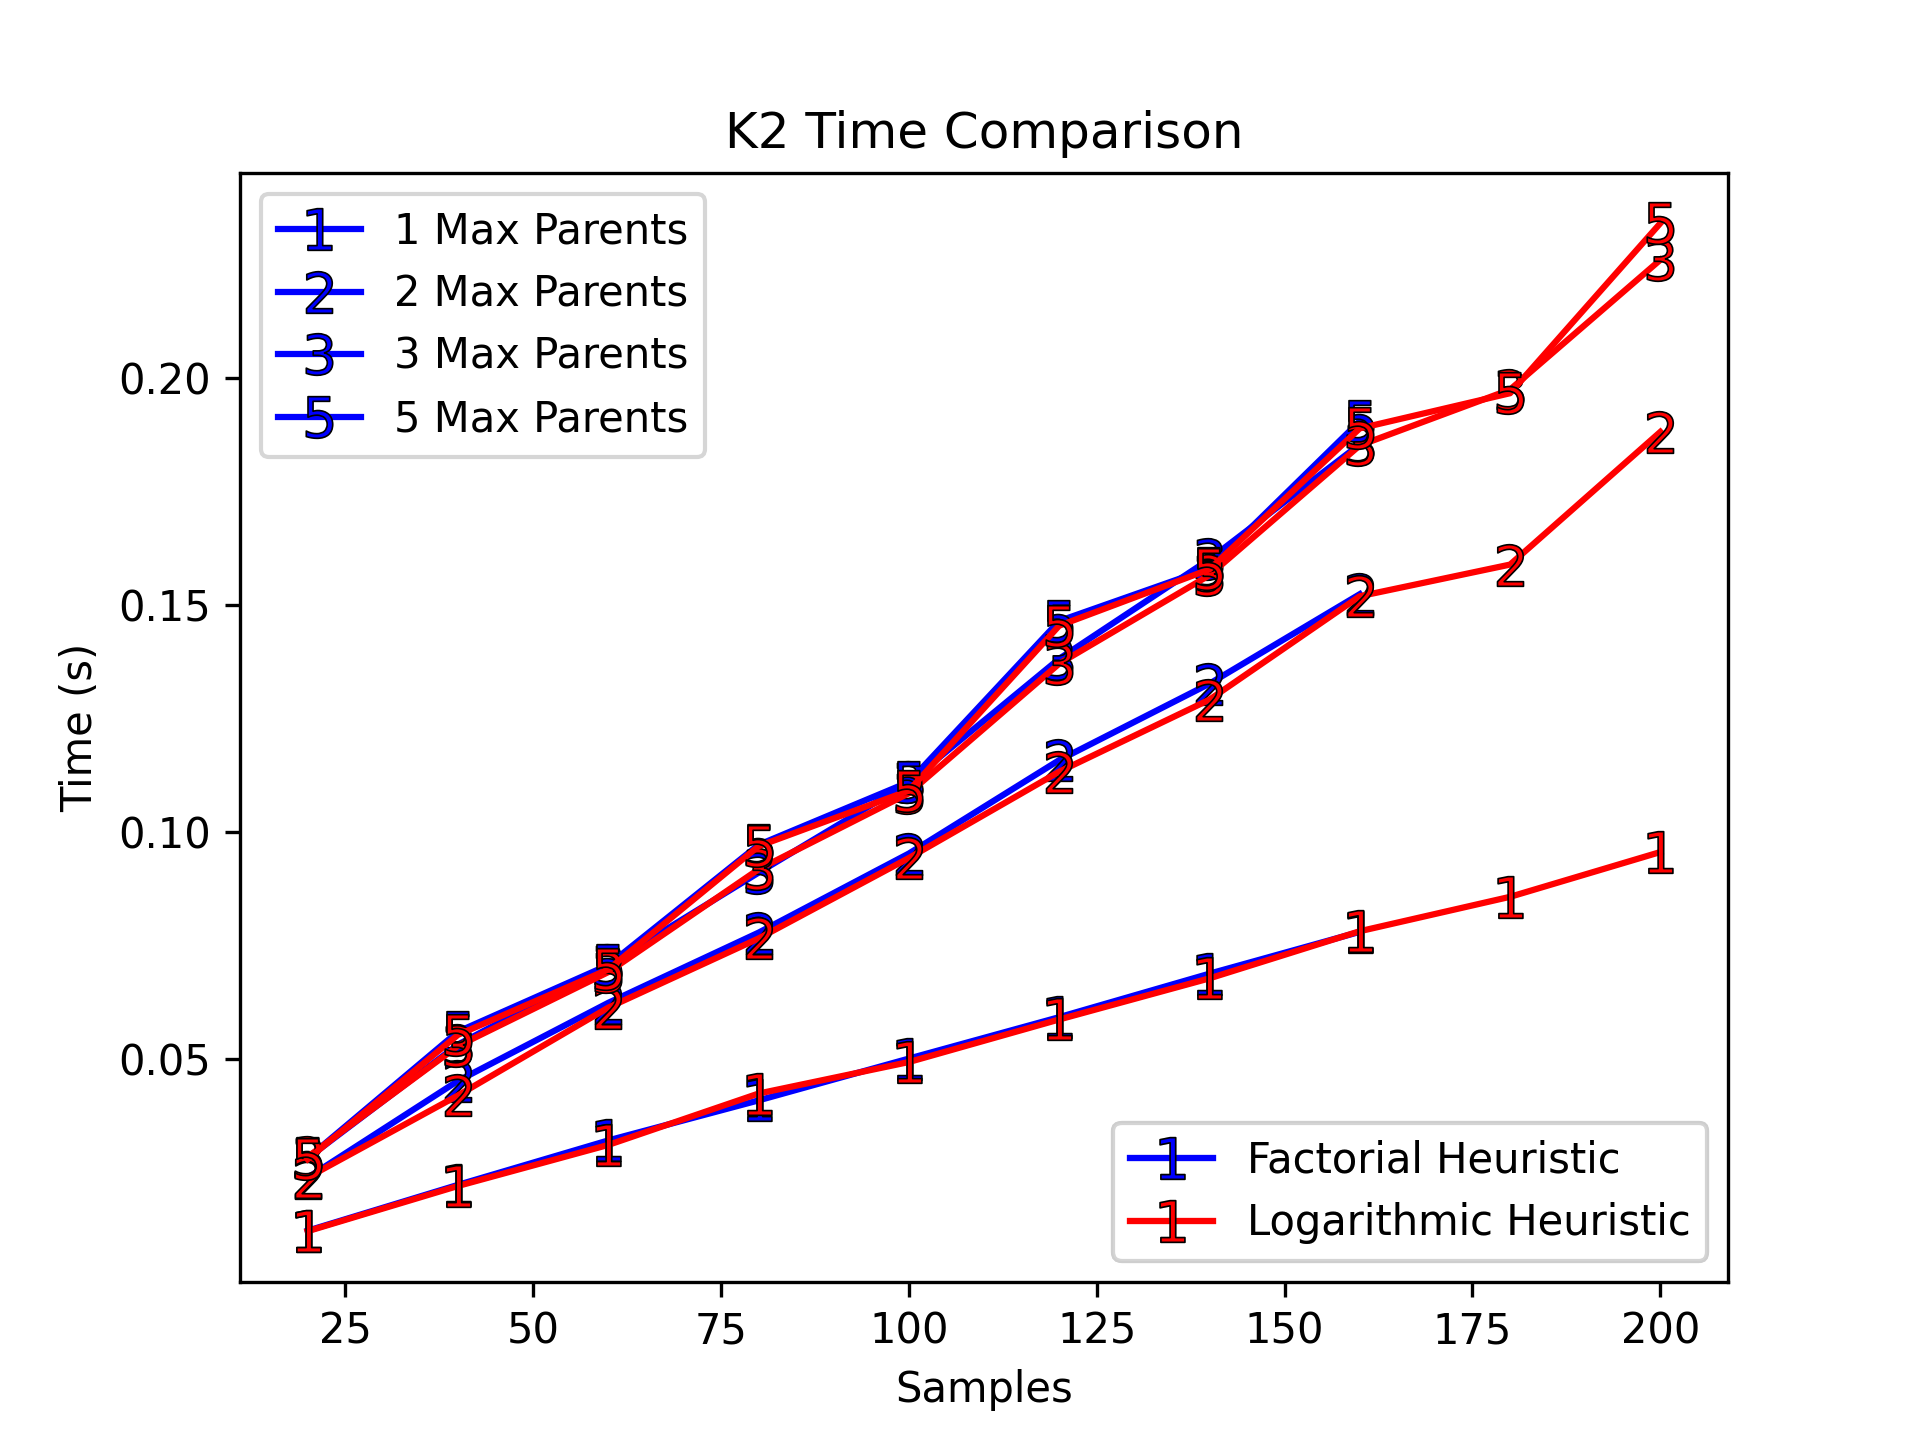
\includegraphics[width=0.75\textwidth]{k2_times.png}
    \caption{grafico che rappresenta i tempi di esecuzione di \textit{K2}}
    \label{fig:test1}
\end{figure}

I risultati sono rappresentati in figura \ref{fig:test1} e in linea con quanto riportato
nell'articolo\footnotemark[3]: i tempi di \textit{K2} risultano lineari rispetto al numero di
campioni, e si può notare che man mano che si aumenta il numero massimo di dipendenze condizionali
i tempi aumentano fino a arrivare a un \textit{plateau}: infatti con massimo uno o due dipendenze
condizionali per nodo notiamo differenze nei tempi, mentre per le curve con massimo tre e cinque
dipendenze non notiamo particolari differenze; questo è dovuto al fatto che la funzione euristica
blocca in anticipo l'estensione del numero dei padri osservando valori della funzione euristica
peggiori. Per quanto riguarda il tipo di funzione euristica applicata non si notano alcune
differenze sui tempi, ma è possibile osservare un'altro fenomeno: oltre 160 campioni l'algorimo con
l'euristica fattoriale fallisce nell'esecuzione per errori di \textit{overflow}, mentre applicando
l'euristica logaritmica non si hanno problemi di questo tipo; questo si spiega dal fatto che la
funzione euristica fattoriale genera punteggi molto bassi in modulo che devono essere moltiplicati
per fattoriali di numeri molto elevati.

